\subsection{\secState{R}Rule Implementation}\label{sec:ruleImplementation}

\paragraph{Configuration:} The \emph{Rule Engine Architecture} (fig. \ref{fig:RuleEngineBasicArchitecture}) is configured to handle \emph{UTM functionality} for \emph{Collision Case Resolution} (sec. \ref{sec:collisionCase}).  The overview of \emph{Context} (Green), \emph{Decision Points} (red) and \emph{Rules to be Invoked} (cyan) is given in (fig. \ref{fig:RuleEngineInstanceLevels}). 

\begin{figure}[H]
    \centering
    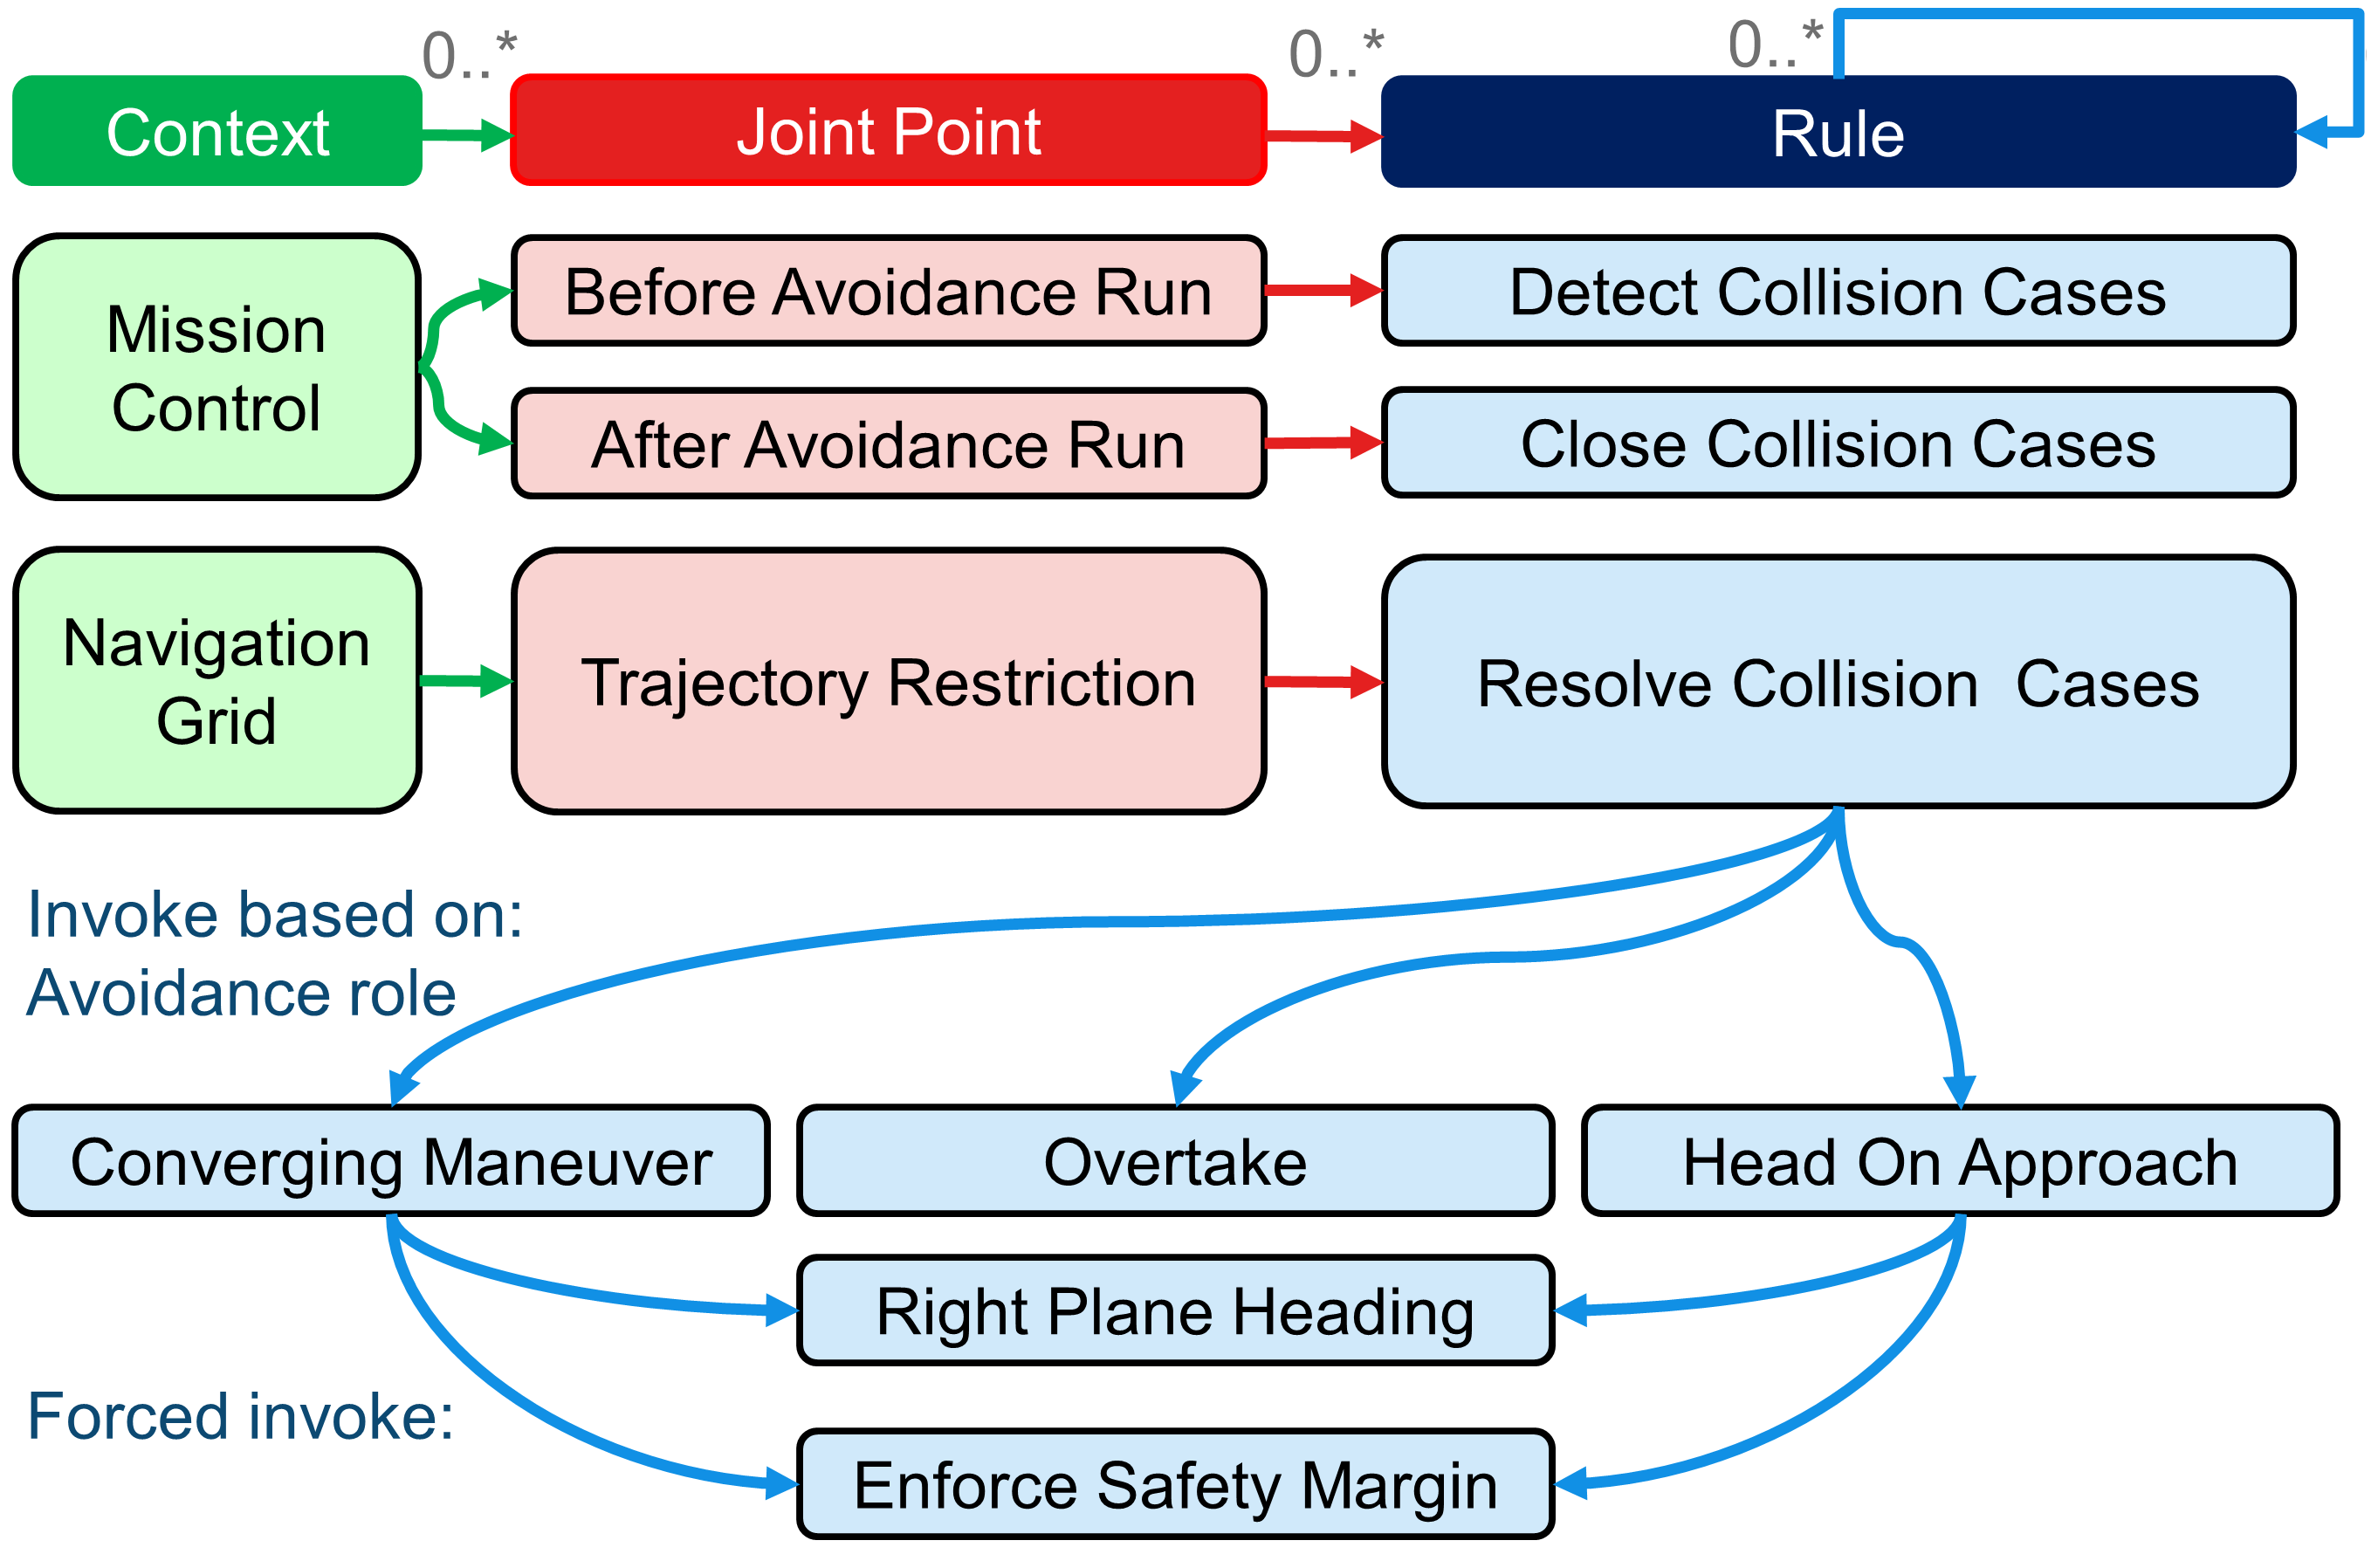
\includegraphics[width=0.7\linewidth]{\FIGDIR/RE014RuleEngineInstanceLevels} 
    \caption{Rule engine initialization with Rules of the air.}
    \label{fig:RuleEngineInstanceLevels}
\end{figure}

\paragraph{Decision Points:} The \emph{Decisions} are bounded to \emph{Mission Control Run Process} (fig. \ref{fig:missionControlRunActivityDiagram}) in following manner:
\begin{enumerate}
    \item \emph{Before Avoidance Run} (before step 7.) - Context: \emph{Mission Control} (Received Collision Cases) - the \emph{UTM} can send  directives. It is required to find which ones are impacting our \emph{UAS}.
    
    \item \emph{Trajectory Restrictions} (after step 7.) - Context: \emph{Navigation Grid} (Trajectory Restrictions) - adaptation of \emph{behavior} imposed by \emph{active collision cases}.
    
    \item \emph{After Avoidance Run} (after step 11.) - Context: \emph{Mission Control} (Collision Case Resolutions) - our \emph{UAS} will update the status of \emph{Collision Cases} then it checks the \emph{avoidance conditions}. The \emph{Resolution Notification} resolution notifications are sent to UTM afterwards.
    
\end{enumerate}

\begin{note}
    The \emph{Weather Case} (sec. \ref{sec:weatherCase}) is handled in similar manner. The mission control loop (fig. \ref{fig:missionControlRunActivityDiagram}) have rules with separate \emph{Decision Points} to enforce \emph{hard constraints} (before step 9.) and \emph{soft constraints} (before step 10.).
\end{note}

\paragraph{Road map:} The \emph{implemented rules}(cyan) are separated into following categories:
\begin{enumerate}
    \item \emph{Management Rules} - managing collision cases (additional control flow):
        \begin{enumerate}[a.]
            
            \item \emph{Detect Collision Cases} (sec. \ref{sec:detectCollisionCases}) - the detection of active participation in received \emph{collision cases} and generation of \emph{restrictions}.
            
            \item \emph{Resolve Collision Cases} (sec. \ref{sec:ruleResolveCollisionCase}) - the enforcement of \emph{active avoidance roles} in \emph{collision cases}. The one \emph{Restriction Rule} is invoked directly.
            
            \item \emph{Close Collision Cases} (sec. \ref{sec:ruleCloseCollisionCases}) - impact calculation and \emph{Resolution Notification} to \emph{UTM} authority.
        \end{enumerate}
    
    \item \emph{Restriction Rules} - restricting the \emph{Navigation Grid} trajectories or altering \emph{goal waypoint} based on \emph{selected collision cases}:
    \begin{enumerate}[a.]
        \item \emph{Converging Maneuver} (sec. \ref{sec:ruleConvergingManuever}) implementation of \emph{Converging Avoidance} (sec. \ref{sec:handlingConvergingManuever}).
        
        \item \emph{Head On Approach} (sec. \ref{sec:ruleHeadOnApproach}) implementation of \emph{Virtual Roundabout Enforcement} (sec. \ref{sec:handlingHeadOnApproach}).
        
        \item \emph{Overtake} (sec. \ref{sec:ruleOvertake}) implementation of \emph{overtake maneuver} for \emph{Overtaking plane} (sec. \ref{sec:handlingOvertakeManuever}).
    \end{enumerate}
    
    \item \emph{Miscellaneous Rules} - reused pieces of code in \emph{Head On} and \emph{Converging Situations}:
    \begin{enumerate}[a.]
        \item \emph{Right Plane Heading} (sec. \ref{sec:ruleRightPlaneHeading}) - restrict all trajectories heading to space separated by parametric plane in \emph{Avoidance Grid} which are heading or belonging to plane.
        
        \item \emph{Enforce Safety Margin} (sec. \ref{sec:ruleEnforceSafetyMargin}) - restrict all \emph{Trajectories Segments} which are in proximity of \emph{Collision Point} lesser than \emph{Enforced Safety Margin}.
    \end{enumerate}
\end{enumerate}